\documentclass[12pt]{article}
\usepackage[margin=1in]{geometry}
\usepackage{graphicx}
\usepackage{amsmath}
\usepackage{lscape}
\usepackage{fancyhdr}
\usepackage{hyperref}
\usepackage{booktabs}

% Setup header
\pagestyle{fancy}
\fancyhf{}
\fancyhead[L]{USC Facilities: Rain Barrel Water Pump System} % Team name in the header
\fancyfoot[C]{\thepage} % Page number in the footer

\begin{document}

\title{
    \vspace{2in}
    \textbf{EMCH427-002} \\[1ex]
    \textbf{Product Specifications Report} \\[1ex]
    \textbf{Sponsor: USC Facilities} \\[1ex]
    \vspace{2in}
}

\author{
    \textbf{Team Members:} \\[2ex]
    Tanner Harmon  \\[1ex]
    Presston McConnell  \\[1ex]
    William Wenzel  \\[1ex]
    Jacob Vaught   \\[2ex]
}

\date{}

\maketitle
\thispagestyle{fancy}

\section*{Product Mission}
\noindent USC Facilities requires a water distribution system that transfers water quickly, provides sufficient pressure for effective delivery, ensures adequate flow for all watering methods, covers the entire garden area efficiently, and complies with relevant safety standards.

\section*{List of All Functions in Approximate Sequential Order}
The essential functions for the water distribution system, as derived from the provided diagrams, are:

\begin{enumerate}
    \item Activation of Transfer[User Input]
    \item Adjustment of Flowrate[User Input]
    \item Storing Water
    \item Transferring Water
    \item Controlling Flowrate
    \item Delivering Water
    \item Irrigating the Garden[Output]
    \item Receiving Power[Energy Requirement]
\end{enumerate}

\subsection*{Functional Diagram}
\begin{figure}[h!]
    \centering
    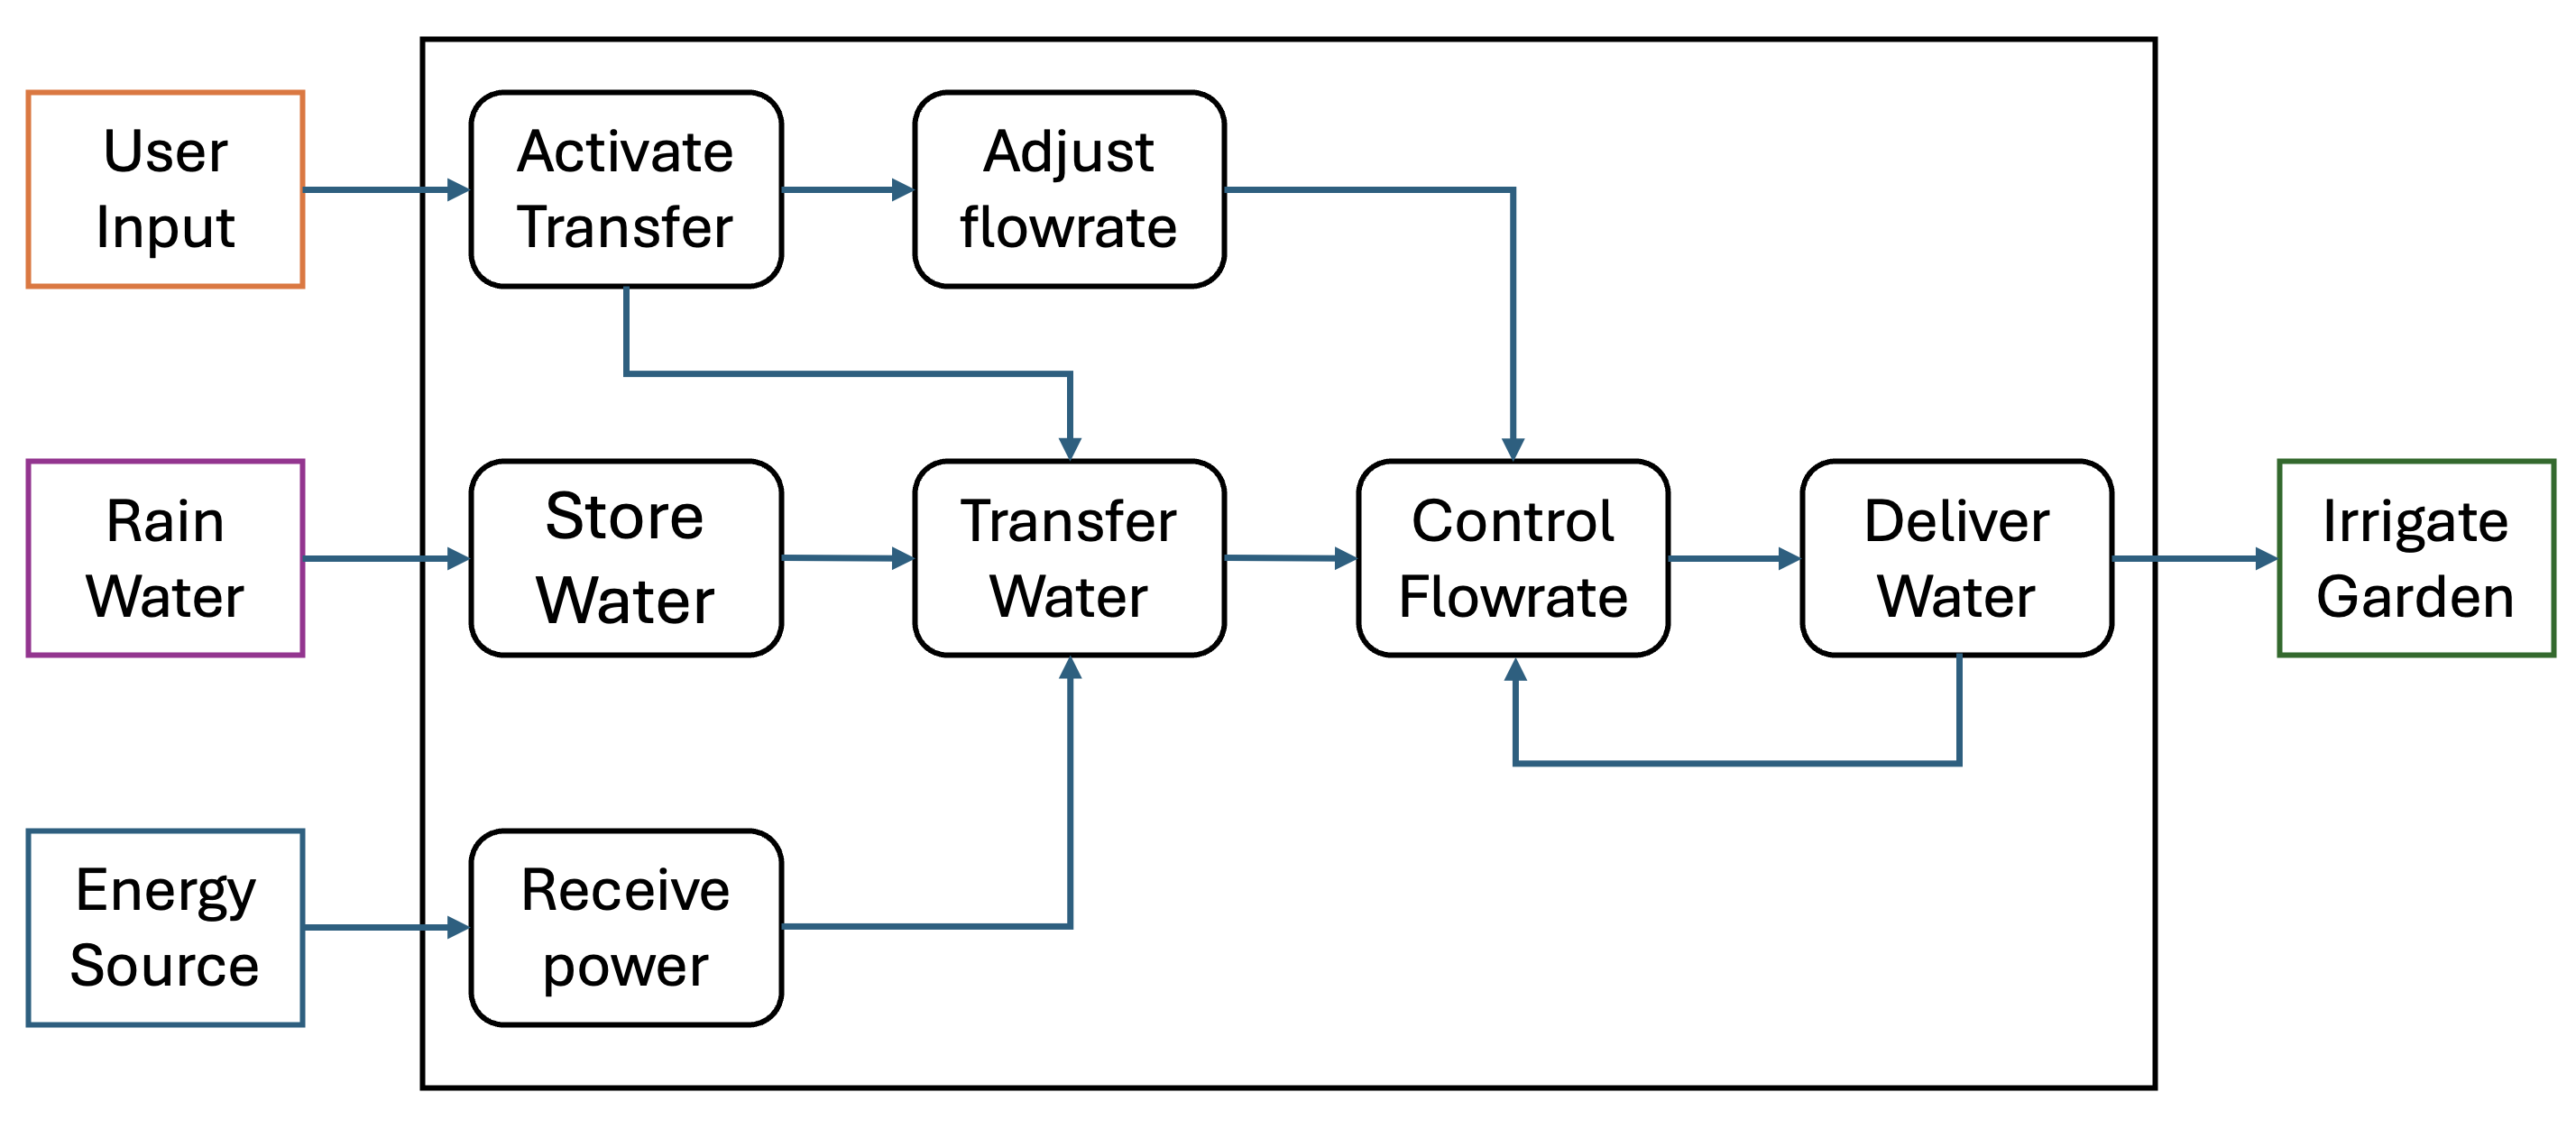
\includegraphics[width=0.8\textwidth]{function_diagram.png}
    \caption{Functional Diagram of the Water Distribution System}
\end{figure}

\begin{figure}[h!]
    \centering
    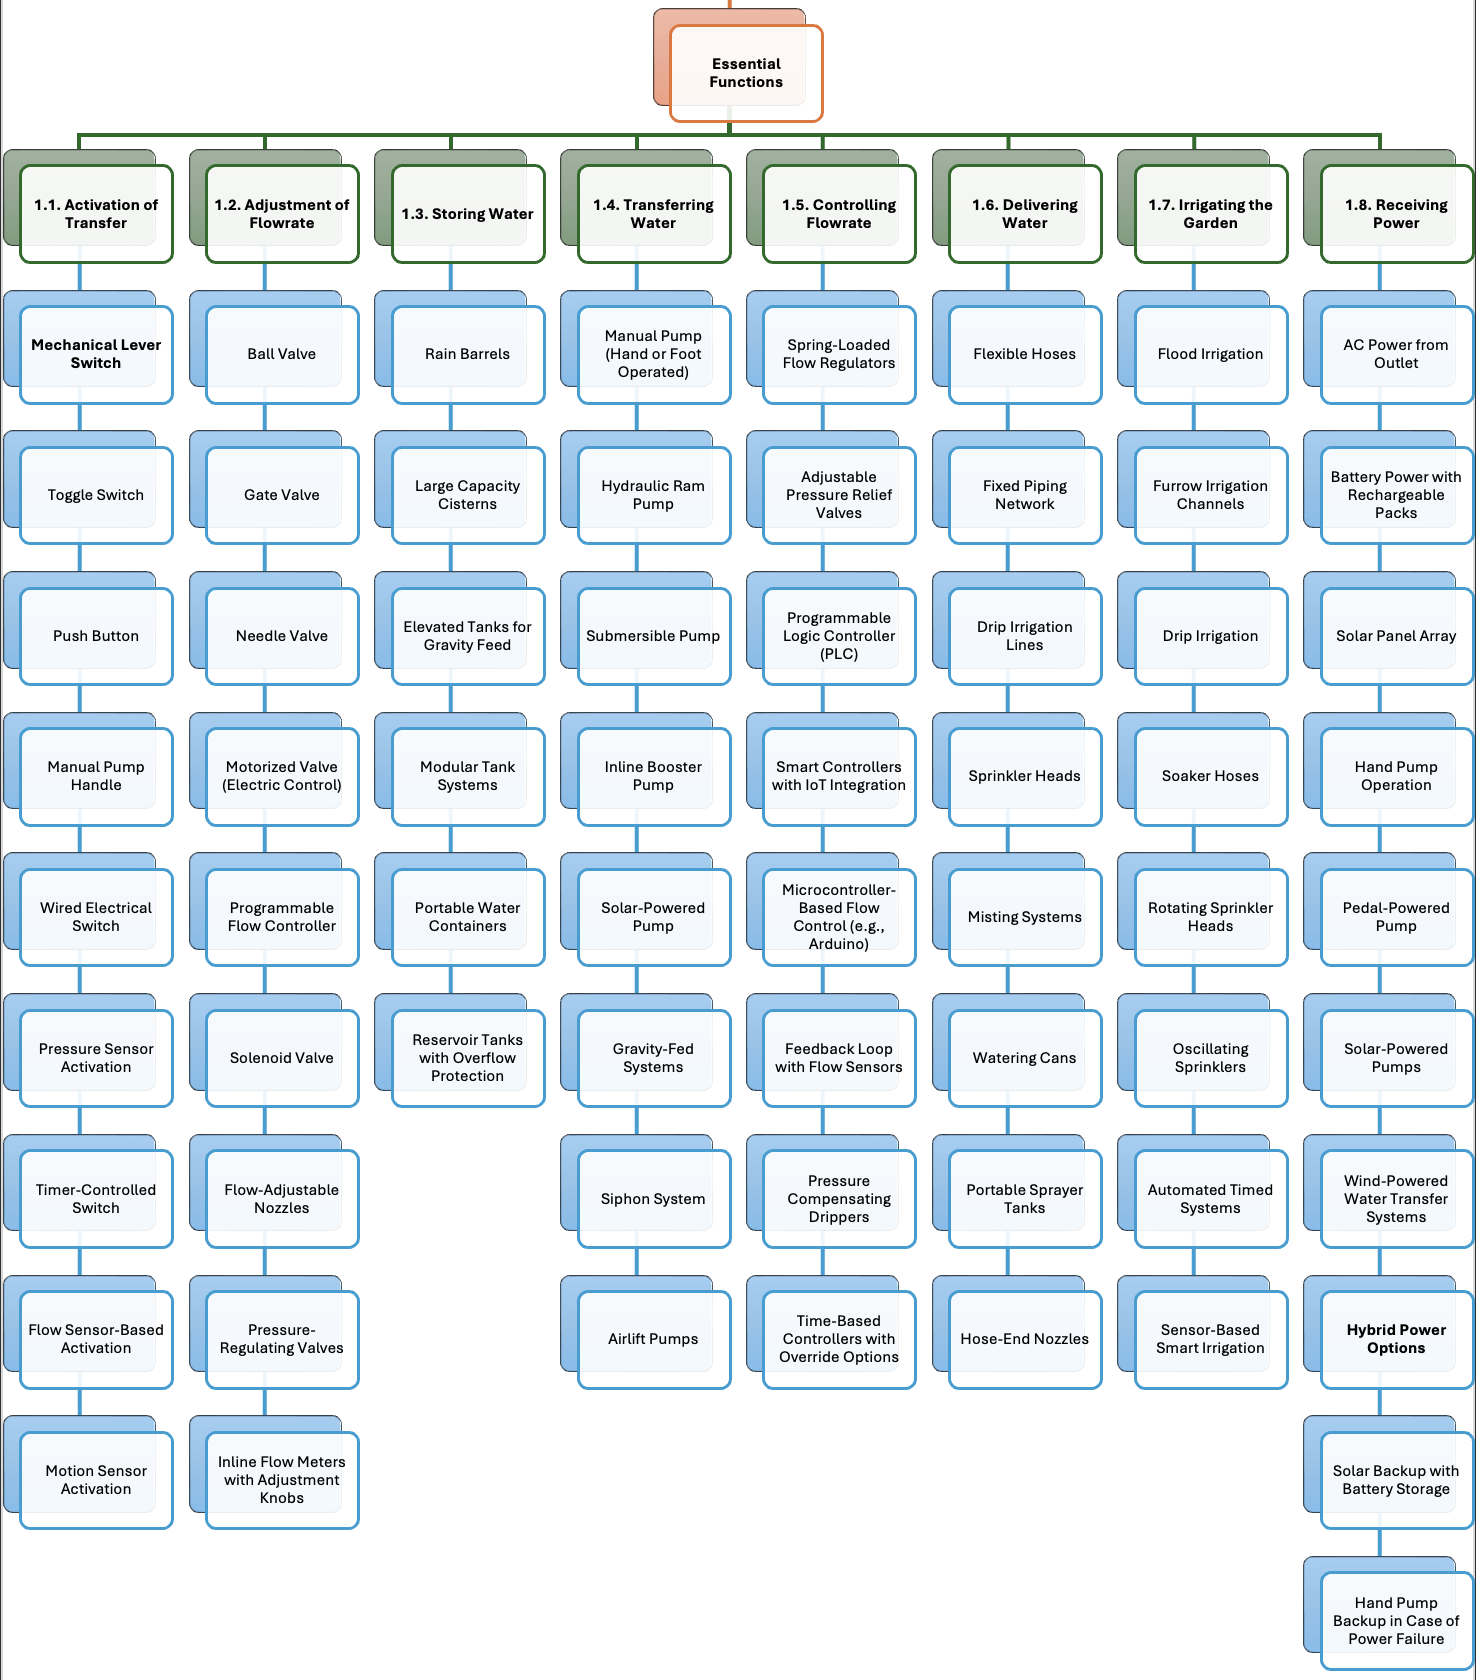
\includegraphics[width=1.0\textwidth]{CCT.png}
    \caption{Concept Combination Table for Water Distribution System Design}
\end{figure}


\end{document}
